\documentclass[border=10pt]{standalone}
\usepackage{tikz}
\usetikzlibrary{shapes.geometric, arrows.meta, positioning, calc, fit, backgrounds}

\begin{document}
\begin{tikzpicture}[
    font=\sffamily,
    >=Stealth,
    node distance=1.4cm and 1.6cm,
    block/.style={draw=teal!70!black, fill=teal!8, line width=1.2pt, rounded corners=4pt, text centered, inner sep=6pt},
    reg/.style={draw=gray!80, fill=gray!20, line width=1pt, rounded corners=2pt, minimum height=2.2cm, minimum width=0.5cm, inner sep=2pt, text centered},
    bus/.style={line width=1.3pt, ->}
]

    % Input
    \node (din) at (0, 2) {\textbf{Input Tile $d$}\\ \small 4 $\times$ 4 INT16 (Signed)};

    % 1D Col Transform
    \node[block, minimum width=4.0cm, minimum height=3.0cm, right=1.5cm of din] (col_trans) {
        \textbf{4 $\times$ 1D Column Transforms}\\
        \textbf{\texttt{input\_transform\_1d}}\\
        \vspace{0.15cm}
        \small $W = B^T \cdot d$\\
        \footnotesize $w_0 = d_0 - d_2$\\
        \footnotesize $w_1 = d_1 + d_2$\\
        \footnotesize $w_2 = d_2 - d_1$\\
        \footnotesize $w_3 = d_1 - d_3$\\
        \vspace{0.1cm}
        \footnotesize Bit-growth: $16 \to 17$ bits
    };

    % Transposition Matrix / Rewiring
    \node[block, fill=orange!8, draw=orange!70!black, minimum width=2.4cm, minimum height=2.6cm, right=1.2cm of col_trans] (transp) {
        \textbf{Spatial Transpose}\\
        \textbf{Rewiring}\\
        \vspace{0.15cm}
        \small $W^T = (B^T d)^T$\\
        \footnotesize Parallel bus permutation\\
        \footnotesize (Zero logic overhead)
    };

    % 1D Row Transform
    \node[block, minimum width=4.0cm, minimum height=3.0cm, right=1.2cm of transp] (row_trans) {
        \textbf{4 $\times$ 1D Row Transforms}\\
        \textbf{\texttt{input\_transform\_1d}}\\
        \vspace{0.15cm}
        \small $V = B^T \cdot W^T$\\
        \footnotesize $v_0 = w_0 - w_2$\\
        \footnotesize $v_1 = w_1 + w_2$\\
        \footnotesize $v_2 = w_2 - w_1$\\
        \footnotesize $v_3 = w_1 - w_3$\\
        \vspace{0.1cm}
        \footnotesize Bit-growth: $17 \to 18$ bits
    };

    % Pipeline Registers
    \node[reg, right=1.2cm of row_trans] (out_reg) {\rotatebox{90}{\textbf{PIPE REG (18b)}}};

    % Output
    \node[right=1.2cm of out_reg] (vout) {\textbf{Transformed Tile $V$}\\ \small 4 $\times$ 4 INT18 (Signed)};

    % Busses
    \draw[bus] (din) -- node[above, font=\footnotesize] {16 $\times$ 16b} (col_trans.west);
    \draw[bus] (col_trans.east) -- node[above, font=\footnotesize] {16 $\times$ 17b} (transp.west);
    \draw[bus] (transp.east) -- node[above, font=\footnotesize] {16 $\times$ 17b} (row_trans.west);
    \draw[bus] (row_trans.east) -- node[above, font=\footnotesize] {16 $\times$ 18b} (out_reg.west);
    \draw[bus] (out_reg.east) -- node[above, font=\footnotesize] {16 $\times$ 18b} (vout.west);

    \begin{scope}[on background layer]
        \node[draw=teal!50, fill=teal!2, dashed, line width=1.4pt, rounded corners=6pt,
              fit=(col_trans) (transp) (row_trans) (out_reg),
              inner sep=14pt,
              label={[font=\bfseries\color{teal!80!black}, anchor=north west]north west:Multiplierless 2D Input Transformation Unit (\texttt{input\_transform\_2d.sv})}] {};
    \end{scope}

\end{tikzpicture}
\end{document}
